\documentclass[11pt]{beamer}
\usetheme{CambridgeUS}
\usepackage[utf8]{inputenc}
\usepackage{subcaption}
\usepackage{amsmath}
\usepackage{amsfonts}
\usepackage{amssymb}
\usepackage{graphicx}
\usepackage{tcolorbox}

\author[CS685]{ \large Group - 7  \\ \medskip  \small  Debanjan Chatterjee - 20111016  \\ P J Leo Evenss - 20111038 \\ Shilpa Chatterjee - 20111057 \\ Shruti Sharma - 20111061  \\Bopanna Tej Kiran - 20111070}
\title{Extreme Rainfall Prediction in India}
\titlegraphic{
\includegraphics[width=1.4cm]{redlogo.jpg}}
\setbeamercovered{transparent} 
\setbeamertemplate{navigation symbols}{} 
\institute[]{Indian Institute of Technology, Kanpur} 
\subject{CS685 - Data Mining} 
\date{\today}

\begin{document}

\begin{frame}
\titlepage
\end{frame}

\begin{frame}{Introduction}
\begin{itemize}
\item The variability of the Indian Summer Monsoon affects the agricultural production, industry, hydroelectric power, and causes severe strain on the national economy.\\

\item Occurrence of extreme rainfall is an important problem in the field of meteorology as it has a enormous impact on the life of people.\\

\item Every year people across the globe suffer from severe consequences of heavy rainfall like flood, spread of diseases, wastage of agricultural produce, loss of life and belongings etc.\\

\item The government of India spends large amount of money to provide relief in the affected areas.
\end{itemize}
\end{frame}

\begin{frame}{Problem Statement}
The available methods for heavy rainfall prediction are able to predict only 6 h prior to the event.\\
 We have tried to address the problem of predicting the occurrence of extreme rainfall events across regions during the summer monsoon months of June-September atleast 48-hour and 24-hour before.\\
 
 \medskip
 
The information of regional and sub-divisional rainfall is very much useful to the Researchers, Policy makers and Governmental agencies. This will ensure that least damage is caused by heavy rainfall events. 
\end{frame}

\begin{frame}{Dataset}
\begin{itemize}
\item Daily data of weather parameters at surface and multiple levels is extracted from NCEP/NCAR reanalysis data. (Latitude - 5\textdegree \ to 40\textdegree \ north,  Longitude - 65\textdegree \ to 100\textdegree \ east)
\item Rainfall data is obtained from India Meteorological Department (IMD, Pune).
\item Total parameters sum to 22.
\item 20 years have been considered for analysis (1997-2016).
\end{itemize}
\end{frame}

\begin{frame}{Weather Variables}
The weather variables this study considers are:
\begin{itemize}
\item Air temperature
\item Mean sea level pressure
\item Precipitable water
\item Relative humidity
\item Vertical wind velocity (omega)
\item U-wind
\item V-wind.
\end{itemize}
Apart from surface level, for multiple levels we have considered weather parameters at 850-, 600- and 400-hPa levels.
\end{frame}

\begin{frame}{Subdivisions}
There are 36 meteorological subdivisions of India.
\begin{figure}
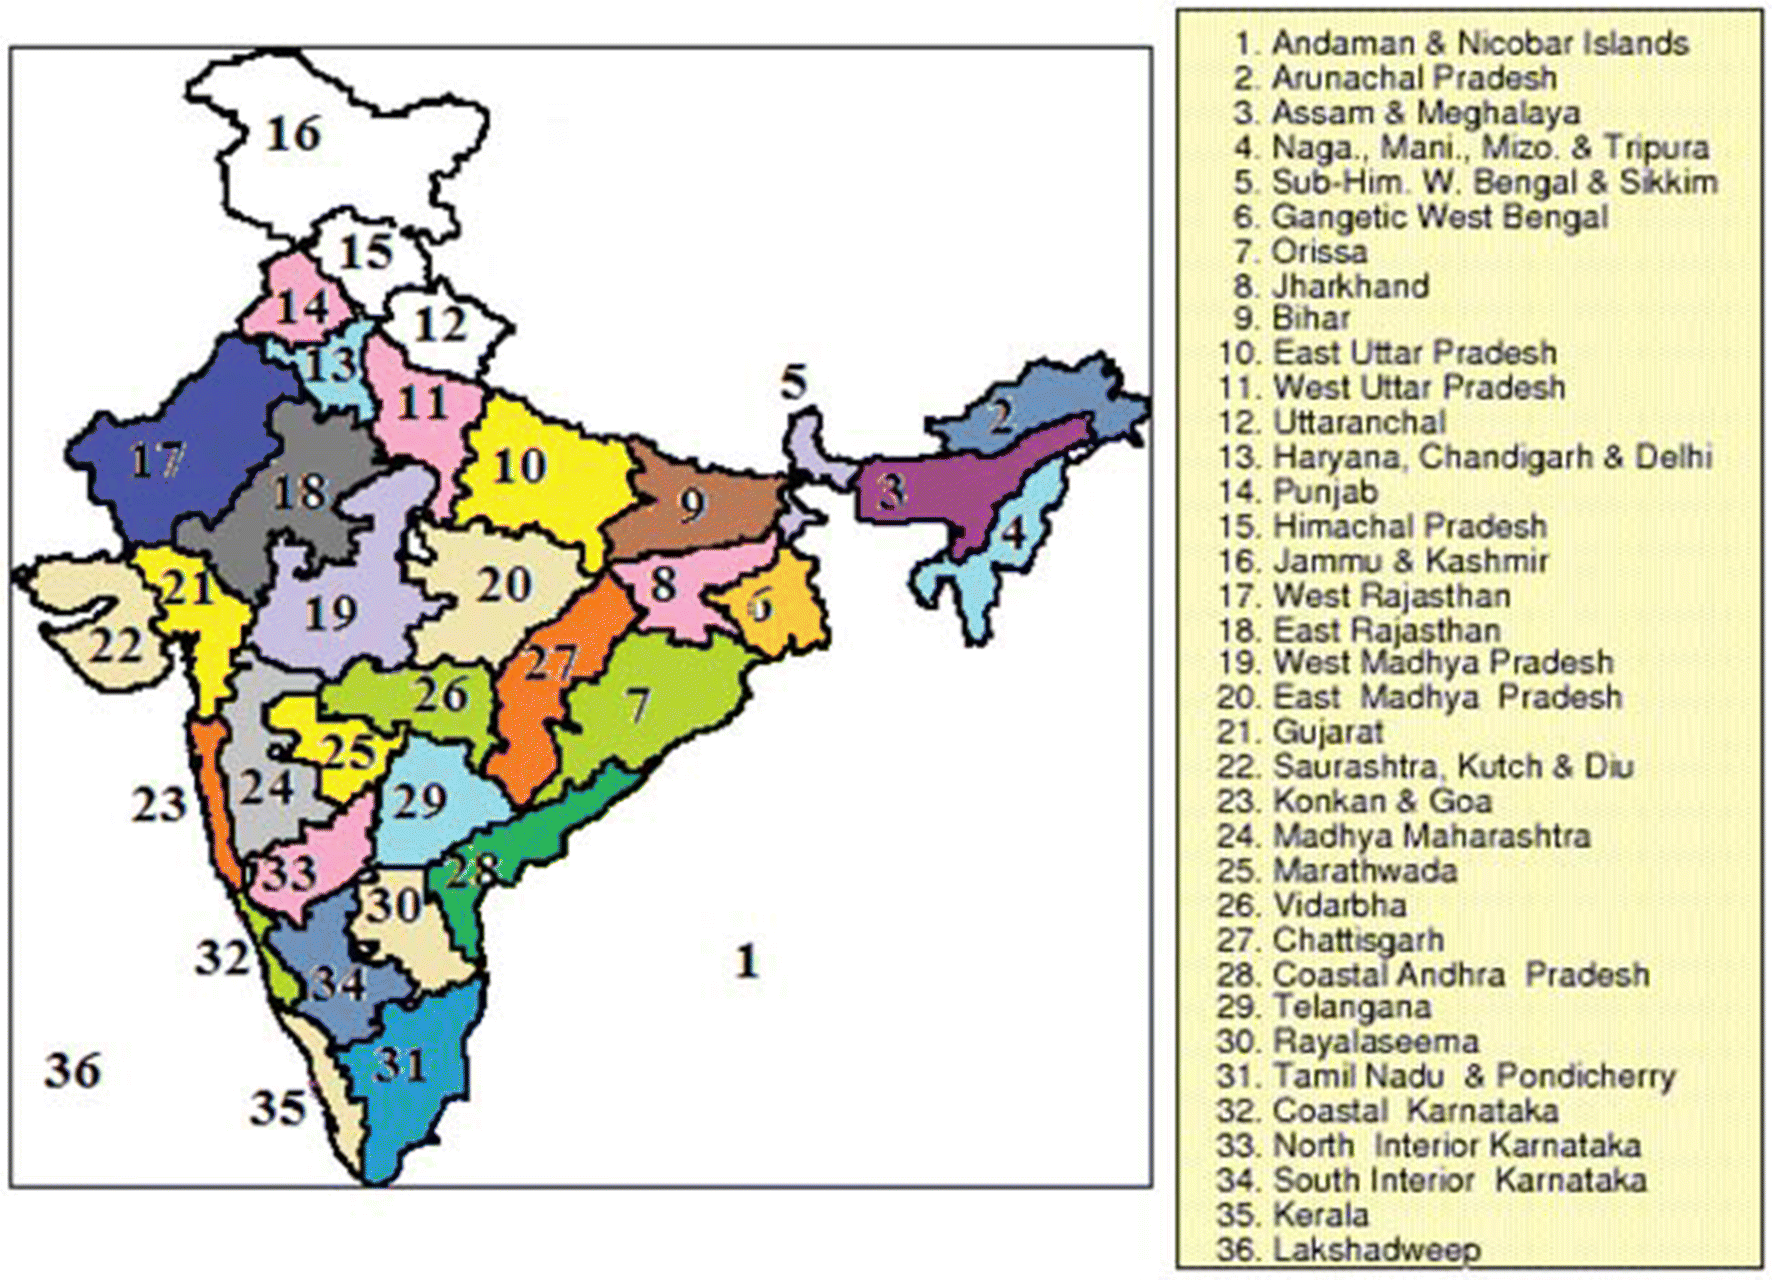
\includegraphics[scale=0.13]{Fig1.png}
\end{figure}
\footnote{\small Image Source: Meteorological Subdivision - OGD Platform India}
\end{frame}

\begin{frame}{Methodology}
\begin{itemize}
\item The validity of any statistical analysis depends on the quality of the data used in the analysis.
\item  Subdivisions are distributed fairly uniformly over the country, so  districts from each subdivision were selected to form the network.
\item A total of 22*225 = 4950 variables available for each day since daily data is taken. For 48 h and 24 h prior prediction, the variables are increased to 4950*2 = 9900. 
\item Missing values are flagged with -9.96921e+36f
\item Excess if \textit{R $>$ or = M+SD}, where M and SD are Mean and Standard Deviation of region's rainfall. R is the region's rainfall.
\end{itemize}
\end{frame}

\begin{frame}{The Beginning}
We started with a set of 7 features namely air temperature, mean sea level pressure, precipitable water, relative humidity, vertical wind velocity (omega), U-wind and V-wind at the surface level  The Indian subcontinent was divided into equi-sized 225 grids and the daily data was prepared from these resulting in 225 * 7 =1575 features per day. The model trained with these features 
resulting in precision = 0.60 and recall = 0.16. \\

The features were then scaled up considering the different air pressure levels of  850-, 600- and 400-hPa and then dataset amounted to 22 feature attributes , thus 225 * 22=4950 per day and 4950 * 2=9900 for 2 consecutive days.
\end{frame}

\begin{frame}{Feature Reduction using Auto-encoders}
Such huge set of features if used for training a machine learning model may lead to overfitting. Therefore, we need a feature reduction technique.\\

\textbf{Architecture of Auto-encoder} -
\begin{itemize}
\item An input layer, (bias b = 9900)
\item 2 hidden layers (initial units W = 2500, bias = 2500),
\item An output layer (bias = 9900)
\item Activation function - Sigmoid
\item Optimizer - Adagrad
\item Learning rate - 0.1
\item Batch size - 100
\item Cost function - MSE
\end{itemize}
The size of encoded features comes out to be 2500 from initial 9900.

\end{frame}

\begin{frame}{SMOTE}
To effectively deal with the class imbalance problem in our biased dataset and to get the best performance, oversampling of minority class has been tackled using SMOTE.

\begin{figure}[!h]
\begin{subfigure}{.5\textwidth}
\centering
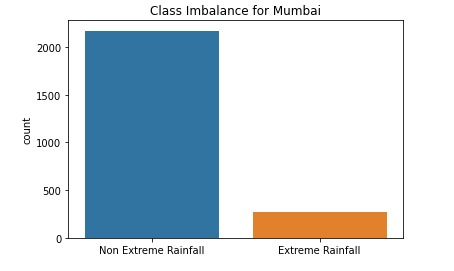
\includegraphics[width=.8\linewidth]{Fig3.jpeg}
\caption{Skewness in Mumbai Rainfall data}
\end{subfigure}%
\begin{subfigure}{.5\textwidth}
\centering
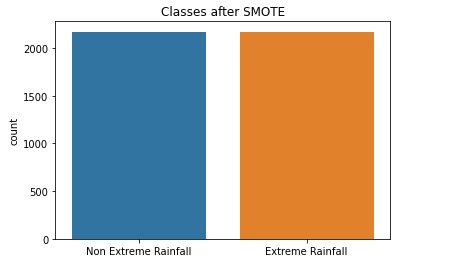
\includegraphics[width=.8\linewidth]{fig4.jpeg}
\caption{After applying SMOTE}
\end{subfigure}
\end{figure}
\end{frame}

\begin{frame}{ROC Curves - Mumbai}
\begin{figure}[!h]
\begin{subfigure}{.5\textwidth}
\centering
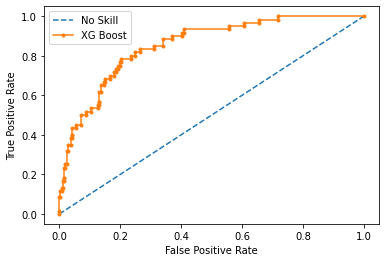
\includegraphics[width=.8\linewidth]{mumbai_normal.png}
\caption{Non SMOTE (0.853)}
\end{subfigure}%
\begin{subfigure}{.5\textwidth}
\centering
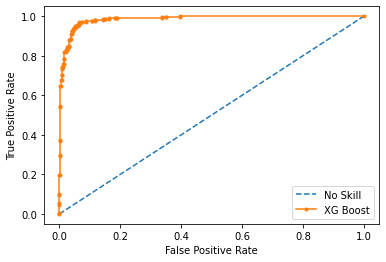
\includegraphics[width=.8\linewidth]{mumbai_smote.png}
\caption{After applying SMOTE (0.99)}
\end{subfigure}
\end{figure}
\end{frame}

\begin{frame}{ROC Curves - Guwahati}
\begin{figure}[!h]
\begin{subfigure}{.5\textwidth}
\centering
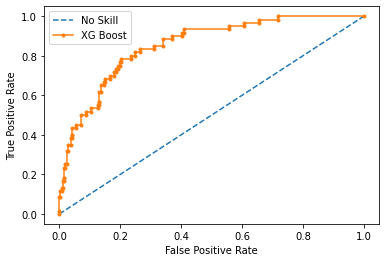
\includegraphics[width=.8\linewidth]{guwahati_normal.png}
\caption{Non SMOTE (0.854)}
\end{subfigure}%
\begin{subfigure}{.5\textwidth}
\centering
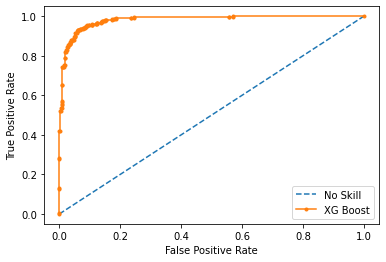
\includegraphics[width=.8\linewidth]{guwahati_smote.png}
\caption{After applying SMOTE (0.981)}
\end{subfigure}
\end{figure}
\end{frame}


\begin{frame}{Results - XGBoost}
\textbf{Auto-encoder + SMOTE + XGB (24 h, Mumbai)} - High recall after dealing with all kinds of problems the data had originally, since Mumbai is one such city that receives heavy rainfall during summer monsoon months.
\begin{figure}[!h]
\begin{subfigure}{.5\textwidth}
\centering
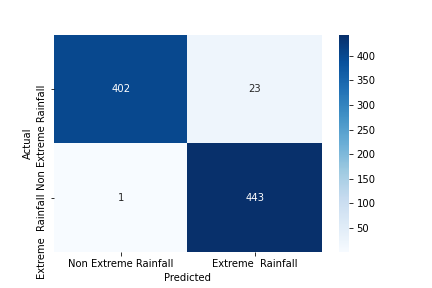
\includegraphics[width=\linewidth]{y_mumbai.png}
\caption{Confusion Matrix}
\end{subfigure}%
\begin{subfigure}{.5\textwidth}
\centering
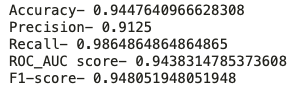
\includegraphics[width=.8\linewidth]{res_mumbai.png}
\caption{Metrics}
\end{subfigure}
\end{figure}
\end{frame}

\begin{frame}{Results - XGBoost}
\textbf{Auto-encoder + XGB (48 h, Mumbai)} - Low recall because of class-imbalance. Also 24 h prediction performs better than 48 h.
\begin{figure}[!h]
\centering
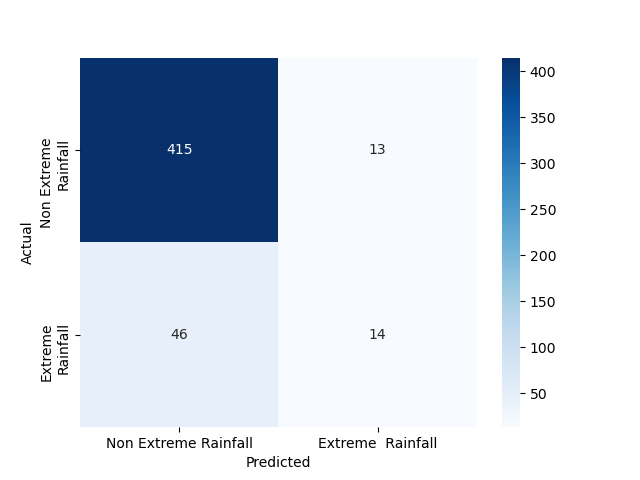
\includegraphics[width=.4\linewidth]{mumbai.png}
\caption{Confusion Matrix}
\end{figure}

\textbf{\small Other Metrics} \begin{itemize}
\item Accuracy - 0.87
\item Precision - 0.51
\item Recall - 0.23, F1-score - 0.32
\end{itemize}
\end{frame}

\begin{frame}{Results - XGBoost} 
\textbf{XGB (24 h, Mumbai)} - Low recall because no preprocessing done to balance the dataset.
\begin{figure}[!h]
\begin{subfigure}{.5\textwidth}
\centering
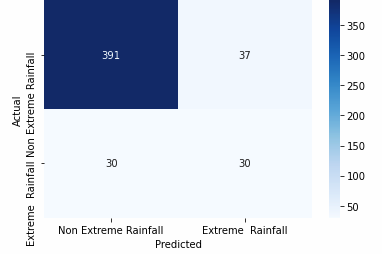
\includegraphics[width=\linewidth]{xgb.png}
\caption{Confusion Matrix}
\end{subfigure}%
\begin{subfigure}{.5\textwidth}
\centering
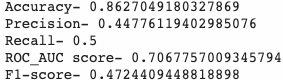
\includegraphics[width=.8\linewidth]{xgb_metrics.png}
\caption{Metrics}
\end{subfigure}
\end{figure}
\end{frame}


\begin{frame}{SVM}
RBF kernel used. 
\begin{figure}[!h]
\begin{subfigure}{.5\textwidth}
\centering
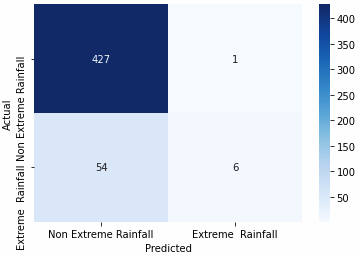
\includegraphics[width=\linewidth]{svm_mumbai.png}
\caption{Confusion Matrix}
\end{subfigure}%
\begin{subfigure}{.5\textwidth}
\centering
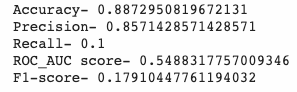
\includegraphics[width=.8\linewidth]{svm_metrics.png}
\caption{Metrics}
\end{subfigure}
\end{figure}
\end{frame}


\begin{frame}{Discussion}
In this work we have explored techniques to learn and represent weather features and use them to predict extreme rainfall events. This model works better because we include all the features and try to understand underlying patterns and dependencies unlike other approaches which rely on selective feature reduction.
\end{frame}

\begin{frame}{Discussion}
\begin{itemize}
\item For the country as a whole, the summer monsoon rainfall do not show any significant trend. However, there are large variations at the regional scale.
\item Increasing parameters from 7 to 22 improved the quality of results to a great extent.
\item 24 h prediction gave better results on average than 48 h prediction.
\item SMOTE gave excellent results.
\item For model without SMOTE, even though a cost-sensitive model was used, the performance of model degraded, especially for cities with low percentage of extreme rainfall days, and thus made the dataset more skewed.
\end{itemize}
\end{frame}

\begin{frame}{External Links}
\textbf{Github} - \\
\url{https://github.com/Shruti-codes/Extreme-Rainfall_Prediction}

\medskip

\textbf{Website} - \\
\url{https://shruti-codes.github.io/ExtremeRainfall/landingpage.html}
\end{frame}

\begin{frame}{Future Work}
Here we have solved only a classification problem where we are only able to predict whether there will be heavy rainfall or not. In future we would also like to predict the amount of rainfall as well with the improved methods.
\end{frame}

\end{document}